% answers.tex —— 2008 年·普通高等学校招生考试·广东卷·文科 · 参考答案与详细解析片段
% 由 tools/generate_projects.py 依来源总账自 2008/2008_数学真题_广东文_试题.md + 2008/2008_数学真题_广东文_解析正文.md + 2008/2008_数学真题_广东文_答案要点.md 生成，勿手改（改源 MD 后重跑）


\begin{gktip}
固定候选 PDF 仅含题面，无答案、解析和评分标准，原卷亦未标注分值；以下为非官方编者独立推导，官方答案字段为空。来源发布者、出版者、版次与官方身份均未核。
\end{gktip}

\begin{answer}
\gksolhead{1}{}

\textbf{题目}：

第二十九届夏季奥林匹克运动会将于 $2008$ 年 $8$ 月 $8$ 日在北京举行，若集合 $A=\{$参加北京奥运会比赛的运动员$\}$，集合 $B=\{$参加北京奥运会比赛的男运动员$\}$，集合 $C=\{$参加北京奥运会比赛的女运动员$\}$，则下列关系正确的是（　）

（A）$A\subseteq B$

（B）$B\subseteq C$

（C）$A\cap B=C$

（D）$B\cup C=A$

\Needspace{4\baselineskip}
\textbf{解析}

男运动员与女运动员的全体就是全部运动员，故 $B\cup C=A$。

其余：$A\subseteq B$ 显然不对；$B\subseteq C$ 不对（男女不相交）；$A\cap B=B\ne C$。

\gkanswer{答案：D。}

\end{answer}
\begin{answer}
\gksolhead{2}{}

\textbf{题目}：

已知 $0<a<2$，复数 $z=a+\mathrm i$（$\mathrm i$ 是虚数单位），则 $|z|$ 的取值范围是（　）

（A）$(1,\sqrt3)$

（B）$(1,\sqrt5)$

（C）$(1,3)$

（D）$(1,5)$

\Needspace{4\baselineskip}
\textbf{解析}

\Needspace{5\baselineskip}
计算如下：

\nopagebreak[4]
\[|z|=\sqrt{a^2+1},\]

$0<a<2$ 时 $1<a^2+1<5$，故 $|z|\in(1,\sqrt5)$。

\gkanswer{答案：B。}

\end{answer}
\begin{answer}
\gksolhead{3}{}

\textbf{题目}：

已知平面向量 $\boldsymbol a=(1,2)$，$\boldsymbol b=(-2,m)$，且 $\boldsymbol a\parallel\boldsymbol b$，则 $2\boldsymbol a+3\boldsymbol b=$（　）

（A）$(-2,-4)$

（B）$(-3,-6)$

（C）$(-4,-8)$

（D）$(-5,-10)$

\Needspace{4\baselineskip}
\textbf{解析}

\Needspace{5\baselineskip}
$\boldsymbol a\parallel\boldsymbol b$ 给出 $1\cdot m-2\cdot(-2)=0$，即 $m=-4$，故 $\boldsymbol b=(-2,-4)$，

\nopagebreak[4]
\[2\boldsymbol a+3\boldsymbol b=(2,4)+(-6,-12)=(-4,-8).\]

\gkanswer{答案：C。}

\end{answer}
\begin{answer}
\gksolhead{4}{}

\textbf{题目}：

记等差数列 $\{a_n\}$ 的前 $n$ 项和为 $S_n$，若 $S_2=4$，$S_4=20$，则该数列的公差 $d=$（　）

（A）$7$

（B）$6$

（C）$3$

（D）$2$

\Needspace{4\baselineskip}
\textbf{解析}

\Needspace{5\baselineskip}
$S_2=2a_1+d=4$，$S_4=4a_1+6d=20$。由第一式 $2a_1=4-d$，代入第二式：

\nopagebreak[4]
\[2(4-d)+6d=20\ \Longrightarrow\ 8+4d=20\ \Longrightarrow\ d=3.\]

\gkanswer{答案：C。}

\end{answer}
\begin{answer}
\gksolhead{5}{}

\textbf{题目}：

已知函数 $f(x)=(1+\cos2x)\sin^2x$，$x\in\mathbf R$，则 $f(x)$ 是（　）

（A）最小正周期为 $\pi$ 的奇函数

（B）最小正周期为 $\pi$ 的偶函数

（C）最小正周期为 $\dfrac{\pi}{2}$ 的奇函数

（D）最小正周期为 $\dfrac{\pi}{2}$ 的偶函数

\Needspace{4\baselineskip}
\textbf{解析}

\Needspace{5\baselineskip}
计算如下：

\nopagebreak[4]
\[f(x)=(1+\cos2x)\sin^2x=2\cos^2x\sin^2x=\frac12\sin^22x=\frac{1-\cos4x}4.\]

最小正周期 $T=\dfrac{2\pi}4=\dfrac{\pi}{2}$，且为偶函数。

\gkanswer{答案：D。}

\end{answer}
\begin{answer}
\gksolhead{6}{}

\textbf{题目}：

经过圆 $x^2+2x+y^2=0$ 的圆心 $C$，且与直线 $x+y=0$ 垂直的直线方程是（　）

（A）$x-y+1=0$

（B）$x-y-1=0$

（C）$x+y-1=0$

（D）$x+y+1=0$

\Needspace{4\baselineskip}
\textbf{解析}

圆化为 $(x+1)^2+y^2=1$，圆心 $C(-1,0)$。

\Needspace{5\baselineskip}
所求直线与 $x+y=0$ 垂直，斜率为 $1$：

\nopagebreak[4]
\[y=x+1,\qquad\text{\text{即} }x-y+1=0.\]

\gkanswer{答案：A。}

\end{answer}
\begin{answer}
\gksolhead{7}{}

\textbf{题目}：

将正三棱柱截去三个角（如图 1 所示 $A$，$B$，$C$ 分别是 $\triangle GHI$ 三边的中点）得到几何体如图 2，则该几何体按图 2 所示方向的侧视图（或称左视图）为（　）
\nopagebreak[4]
\begin{center}% 2008 年广东卷文科第 7 题：正三棱柱截去三个角前后的图 1、图 2，以及四个侧视图选项。
% 来源 PDF：gaokaomath-src/普通高考/2008/2008广东文.pdf
% SHA-256：1adedadb12b82b7b4d04721908bd686e747021593ec91da14b0e4e979929373c
% 原页：2008广东文.pdf 第 1 页（A3 三栏）第 1 栏，书页码 447。
% 重绘依据：图 1 为正三棱柱 GHI-EFD（H、G 在后，I 在前），A、B、C 分别是 HG、HI、GI 的中点，
%   截角平面为 ABE、ACD、BCF，故新增棱 AB、AC、BC、BE、CD、BF、CF，被遮挡的 AE、AD、ED 用虚线；
%   图 2 为截角后的几何体，只剩 A、B、C、D、E、F 六个顶点，实线为 AB、AC、BC、BE、CD、BF、CF、
%   EF、FD，虚线为 AE、AD、ED。
\begin{tikzpicture}[semithick, font=\small, every node/.style={inner sep=1.2pt}]

  % ---------------- 图 1：正三棱柱 GHI-EFD 与截角线 ----------------
  \begin{scope}[shift={(0,0)}]
    \coordinate (H) at (0,3.45);
    \coordinate (A) at (1.90,3.45);
    \coordinate (G) at (3.80,3.45);
    \coordinate (I) at (1.90,2.15);
    \coordinate (B) at (0.95,2.80);
    \coordinate (C) at (2.85,2.80);
    \coordinate (E) at (0,0.40);
    \coordinate (D) at (3.80,0.40);
    \coordinate (F) at (1.90,-0.85);

    % 可见棱
    \draw (H) -- (G);
    \draw (H) -- (B);
    \draw (G) -- (C);
    \draw (H) -- (E);
    \draw (G) -- (D);
    \draw (B) -- (I) -- (C);
    \draw (I) -- (F);
    \draw (E) -- (F) -- (D);
    % 截角线（可见部分）
    \draw (A) -- (B);
    \draw (A) -- (C);
    \draw (B) -- (C);
    \draw (B) -- (E);
    \draw (C) -- (D);
    \draw (B) -- (F);
    \draw (C) -- (F);
    % 被遮挡的截角线与底边
    \draw[dashed] (A) -- (E);
    \draw[dashed] (A) -- (D);
    \draw[dashed] (E) -- (D);

    \node[above] at (H) {$H$};
    \node[above] at (A) {$A$};
    \node[above] at (G) {$G$};
    \node[below left=1pt] at (B) {$B$};
    \node[below right=1pt] at (C) {$C$};
    \node[right=3pt] at (I) {$I$};
    \node[left] at (E) {$E$};
    \node[right] at (D) {$D$};
    \node[below] at (F) {$F$};
    \node at (1.90,-1.75) {图 1};
  \end{scope}

  % 侧视方向箭头
  \draw[->,>=stealth] (4.45,1.55) -- (5.45,1.55);
  \node[above] at (4.95,1.55) {侧视};

  % ---------------- 图 2：截角后的几何体 ----------------
  \begin{scope}[shift={(6.55,-0.05)}]
    \coordinate (A2) at (1.90,3.35);
    \coordinate (B2) at (0.95,2.62);
    \coordinate (C2) at (2.85,2.62);
    \coordinate (E2) at (0.10,0.30);
    \coordinate (D2) at (3.70,0.30);
    \coordinate (F2) at (1.90,-0.95);

    % 可见棱
    \draw (A2) -- (B2) -- (C2) -- cycle;
    \draw (B2) -- (E2);
    \draw (C2) -- (D2);
    \draw (B2) -- (F2);
    \draw (C2) -- (F2);
    \draw (E2) -- (F2) -- (D2);
    % 被遮挡的棱
    \draw[dashed] (A2) -- (E2);
    \draw[dashed] (A2) -- (D2);
    \draw[dashed] (E2) -- (D2);

    \node[above] at (A2) {$A$};
    \node[below left=1pt] at (B2) {$B$};
    \node[below right=1pt] at (C2) {$C$};
    \node[left] at (E2) {$E$};
    \node[right] at (D2) {$D$};
    \node[below] at (F2) {$F$};
    \node at (1.90,-1.75) {图 2};
  \end{scope}

  % ---------------- 四个侧视图选项 ----------------
  % (A) 左边竖直、顶边半宽、右侧斜边，内部连 E—B
  \begin{scope}[shift={(0,-6.10)}]
    \draw (0,0) -- (0,2.60) -- (1.20,2.60) -- (2.60,0) -- cycle;
    \draw (0,0) -- (1.20,2.60);
    \node[above] at (1.20,2.60) {$B$};
    \node[left] at (0,0) {$E$};
    \node at (1.30,-0.55) {(A)};
  \end{scope}
  % (B) 两侧均为斜边，B 在顶边右端，内部连 E—B
  \begin{scope}[shift={(4.60,-6.10)}]
    \draw (0,0) -- (0.90,2.40) -- (1.55,2.40) -- (2.60,0) -- cycle;
    \draw (0,0) -- (1.55,2.40);
    \node[above] at (1.55,2.40) {$B$};
    \node[left] at (0,0) {$E$};
    \node at (1.30,-0.55) {(B)};
  \end{scope}
  % (C) 右边竖直、左侧斜边，内部连 E—右上角
  \begin{scope}[shift={(0,-9.70)}]
    \draw (0,0) -- (0.90,2.60) -- (2.60,2.60) -- (2.60,0) -- cycle;
    \draw (0,0) -- (2.60,2.60);
    \node[above left] at (0.90,2.60) {$B$};
    \node[left] at (0,0) {$E$};
    \node at (1.30,-0.55) {(C)};
  \end{scope}
  % (D) 两侧均为斜边、整体更窄，B 在顶边右端，内部连 E—B
  \begin{scope}[shift={(4.60,-9.70)}]
    \draw (0,0) -- (0.45,2.40) -- (1.05,2.40) -- (2.60,0) -- cycle;
    \draw (0,0) -- (1.05,2.40);
    \node[above] at (1.05,2.40) {$B$};
    \node[left] at (0,0) {$E$};
    \node at (1.30,-0.55) {(D)};
  \end{scope}
\end{tikzpicture}
\end{center}
\nopagebreak[4]
\Needspace{4\baselineskip}
\textbf{解析}

设底面正三角形边长为 $a$，棱柱高为 $H$。沿图中箭头方向作正投影（与 $BD$ 方向垂直的水平方向）：

底面 $DEF$ 投影为长 $\dfrac{\sqrt3}2a$ 的水平线段（$E$，$D$ 投影重合于左端，$F$ 在右端）；顶面 $ABC$ 是 $GHI$ 的中点三角形，投影为长 $\dfrac{\sqrt3}4a$ 的水平线段，且左端与底面的左端重合。

故侧视图的轮廓是：左边竖直（长 $H$）、上边水平（长 $\dfrac{\sqrt3}4a$）、右边为从顶面右端到底面右端的斜边、下边水平（长 $\dfrac{\sqrt3}2a$）；又 $EB$ 是截角面的一条棱，投影为从下边左端到上边右端的连线。

四条轮廓与内部连线均符合的只有 (A)。

\gkanswer{答案：A。}

\end{answer}
\begin{answer}
\gksolhead{8}{}

\textbf{题目}：

命题“若函数 $f(x)=\log_ax$（$a>0$，$a\neq1$）在其定义域内是减函数，则 $\log_a2<0$”的逆否命题是（　）

（A）若 $\log_a2<0$，则函数 $f(x)=\log_ax$（$a>0$，$a\neq1$）在其定义域内不是减函数

（B）若 $\log_a2\geqslant0$，则函数 $f(x)=\log_ax$（$a>0$，$a\neq1$）在其定义域内不是减函数

（C）若 $\log_a2<0$，则函数 $f(x)=\log_ax$（$a>0$，$a\neq1$）在其定义域内是减函数

（D）若 $\log_a2\geqslant0$，则函数 $f(x)=\log_ax$（$a>0$，$a\neq1$）在其定义域内是减函数

\Needspace{4\baselineskip}
\textbf{解析}

原命题：若 $f$ 在定义域内是减函数，则 $\log_a2<0$。

\Needspace{5\baselineskip}
逆否命题把条件与结论互换并同时否定：

\nopagebreak[4]
\[\text{\text{若} }\log_a2\geqslant0\text{\text{，则} }f(x)=\log_ax\text{ \text{在其定义域内不是减函数}}.\]

\gkanswer{答案：B。}

\end{answer}
\begin{answer}
\gksolhead{9}{}

\textbf{题目}：

设 $a\in\mathbf R$，若函数 $y=\mathrm e^x+ax$，$x\in\mathbf R$ 有大于零的极值点，则（　）

（A）$a<-1$

（B）$a>-1$

（C）$a>-\dfrac1{\mathrm e}$

（D）$a<-\dfrac1{\mathrm e}$

\Needspace{4\baselineskip}
\textbf{解析}

\Needspace{5\baselineskip}
计算如下：

\nopagebreak[4]
\[y'=\mathrm e^x+a.\]

\Needspace{5\baselineskip}
有极值点需 $\mathrm e^x=-a$，即 $a<0$，且极值点 $x=\ln(-a)>0$，故 $-a>1$，

\nopagebreak[4]
\[a<-1.\]

\gkanswer{答案：A。}

\end{answer}
\begin{answer}
\gksolhead{10}{}

\textbf{题目}：

设 $a$，$b\in\mathbf R$，若 $a-|b|>0$，则下列不等式中正确的是（　）

（A）$b-a>0$

（B）$a^3+b^3<0$

（C）$b+a>0$

（D）$a^2-b^2<0$

\Needspace{4\baselineskip}
\textbf{解析}

$a-|b|>0$ 即 $a>|b|\geqslant0$。

于是 $a+b\geqslant a-|b|>0$，即 $b+a>0$ 正确。

其余：(A) $b-a\leqslant|b|-a<0$；(B) 由 $a>|b|$ 得 $a^3>|b|^3\geqslant-b^3$，故 $a^3+b^3>0$；(D) $a^2>b^2$，故 $a^2-b^2>0$。均不正确。

\gkanswer{答案：C。}

\end{answer}
\begin{answer}
\gksolhead{11}{}

\textbf{题目}：

为了调查某厂工人生产某种产品的能力，随机抽查了 $20$ 位工人某天生产该产品的数量。产品数量的分组区间为 $[45,55)$，$[55,65)$，$[65,75)$，$[75,85)$，$[85,95)$，由此得到频率分布直方图如图，则这 $20$ 名工人中一天生产该产品数量在 $[55,75)$ 的人数是\gkblank{}。
\nopagebreak[4]
\begin{center}% 2008 年广东卷文科第 11 题：频率分布直方图。
% 来源 PDF：gaokaomath-src/普通高考/2008/2008广东文.pdf
% SHA-256：1adedadb12b82b7b4d04721908bd686e747021593ec91da14b0e4e979929373c
% 原页：2008广东文.pdf 第 1 页（A3 三栏）第 2 栏，书页码 447。
% 重绘依据：横轴在 0 与 45 之间断开，组距 10；五组 [45,55)、[55,65)、[65,75)、[75,85)、
%   [85,95) 的“频率/组距”依次为 0.020、0.040、0.025、0.010、0.005，纵轴每 0.005 一格并配虚线。
\begin{tikzpicture}[x=1.0cm, y=148cm, semithick, font=\small,
  every node/.style={inner sep=1.2pt}]
  % 坐标轴
  \draw[->,>=stealth] (0,0) -- (12.0,0) node[right] {产品数量};
  \draw[->,>=stealth] (0,0) -- (0,0.0448) node[above] {$\dfrac{\text{频率}}{\text{组距}}$};
  \node[below left] at (0,0) {$0$};

  % 横轴断裂符号
  \draw (0.18,0) -- (0.30,0.0024) -- (0.42,0) -- (0.54,0.0024) -- (0.66,0);

  % 纵轴刻度与水平虚线
  \foreach \h/\lab in {%
    0.005/0.005, 0.010/0.010, 0.015/0.015, 0.020/0.020,
    0.025/0.025, 0.030/0.030, 0.035/0.035, 0.040/0.040} {
    \draw (0,\h) -- (-0.12,\h);
    \node[left] at (-0.12,\h) {\lab};
    \draw[dashed] (0,\h) -- (11.4,\h);
  }

  % 横轴刻度
  \foreach \x/\lab in {1/45, 3/55, 5/65, 7/75, 9/85, 11/95} {
    \draw (\x,0) -- (\x,-0.0024);
    \node[below] at (\x,-0.0024) {\lab};
  }

  % 各矩形（宽 10，高为频率/组距）
  \draw (1,0) rectangle (3,0.020);
  \draw (3,0) rectangle (5,0.040);
  \draw (5,0) rectangle (7,0.025);
  \draw (7,0) rectangle (9,0.010);
  \draw (9,0) rectangle (11,0.005);
\end{tikzpicture}
\end{center}
\nopagebreak[4]
\Needspace{4\baselineskip}
\textbf{解析}

\Needspace{5\baselineskip}
各组的频率为“矩形高 $\times$ 组距 $10$”：

\nopagebreak[4]
\[0.020\times10=0.2,\quad 0.040\times10=0.4,\quad 0.025\times10=0.25,\]

\nopagebreak[4]
\[0.010\times10=0.1,\quad 0.005\times10=0.05,\]

合计 $1$，与总体为 $1$ 相符。

\Needspace{5\baselineskip}
$[55,75)$ 对应第二、三组，频率

\nopagebreak[4]
\[0.4+0.25=0.65,\]

故人数为 $20\times0.65=13$。

\gkanswer{答案：$13$。}

\end{answer}
\begin{answer}
\gksolhead{12}{}

\textbf{题目}：

若变量 $x$，$y$ 满足 $\begin{cases}2x+y\leqslant40,\\ x+2y\leqslant50,\\ x\geqslant0,\\ y\geqslant0,\end{cases}$ 则 $z=3x+2y$ 的最大值是\gkblank{}。

\Needspace{4\baselineskip}
\textbf{解析}

\Needspace{5\baselineskip}
可行域顶点为 $(0,0)$，$(20,0)$，$(0,25)$，以及 $2x+y=40$ 与 $x+2y=50$ 的交点 $(10,20)$。

\nopagebreak[4]
\[z=3x+2y\ \Rightarrow\ 0,\ 60,\ 50,\ 70,\]

故最大值为 $70$。

\gkanswer{答案：$70$。}

\end{answer}
\begin{answer}
\gksolhead{13}{}

\textbf{题目}：

阅读如图的程序框图。若输入 $m=4$，$n=3$，则输出 $a=$\gkblank{}，$i=$\gkblank{}。（注：框图中的赋值符号“$=$”也可以写成“$\leftarrow$”或“$:=$”）
\nopagebreak[4]
\begin{center}% 2008 年广东卷文科第 13 题：程序框图。
% 来源 PDF：gaokaomath-src/普通高考/2008/2008广东文.pdf
% SHA-256：1adedadb12b82b7b4d04721908bd686e747021593ec91da14b0e4e979929373c
% 原页：2008广东文.pdf 第 1 页（A3 三栏）第 3 栏，书页码 447。
% 逻辑：开始→输入 m,n→i=1→a=m×i→判断“n 整除 a?”；
%   是→输出 a,i→结束；否→i=i+1→回到 a=m×i。
\begin{tikzpicture}[>=stealth, semithick, font=\small,
  every node/.style={inner sep=2pt},
  box/.style={draw, minimum width=2.2cm, minimum height=0.7cm},
  term/.style={draw, rounded corners=6pt, minimum width=1.6cm, minimum height=0.6cm},
  io/.style={draw, trapezium, trapezium left angle=110, trapezium right angle=70,
             minimum width=2.6cm, minimum height=0.7cm},
  dec/.style={draw, diamond, aspect=1.9, minimum width=3.0cm, minimum height=1.0cm}]

  \node[term] (s) at (0,0) {开始};
  \node[io]   (in) at (0,-1.2) {输入 $m$，$n$};
  \node[box]  (ini) at (0,-2.3) {$i=1$};
  \node[box]  (mul) at (0,-3.5) {$a=m\times i$};
  \node[dec]  (jud) at (0,-5.0) {$n$ 整除 $a$?};
  \node[box]  (inc) at (3.6,-3.5) {$i=i+1$};
  \node[io]   (out) at (0,-6.5) {输出 $a$，$i$};
  \node[term] (end) at (0,-7.7) {结束};

  \draw[->] (s) -- (in);
  \draw[->] (in) -- (ini);
  \draw[->] (ini) -- (mul);
  \draw[->] (mul) -- (jud);
  \draw[->] (jud) -- node[right] {是} (out);
  \draw[->] (out) -- (end);
  % 否：判断框右侧进入 i=i+1
  \draw[->] (jud.east) -- node[above right] {否} (inc.west);
  % 回路：i=i+1 → 上 → 左 → 下，从右侧回到 a=m×i
  \draw[->] (inc.north) -- (3.6,-2.85) -- (1.35,-2.85) -- (1.35,-3.5) -- (mul.east);
\end{tikzpicture}
\end{center}
\nopagebreak[4]
\Needspace{4\baselineskip}
\textbf{解析}

$i=1$：$a=4$，$3\nmid4$，$i=2$；

$i=2$：$a=8$，$3\nmid8$，$i=3$；

$i=3$：$a=12$，$3\mid12$，输出 $a=12$，$i=3$。

\gkanswer{答案：$a=12$，$i=3$。}

\end{answer}
\begin{answer}
\gksolhead{14}{}

\textbf{题目}：

已知曲线 $C_1$，$C_2$ 的极坐标方程分别为 $\rho\cos\theta=3$，$\rho=4\cos\theta$（$\rho\geqslant0$，$0\leqslant\theta<\dfrac{\pi}{2}$），则曲线 $C_1$ 与 $C_2$ 交点的极坐标为\gkblank{}。

\Needspace{4\baselineskip}
\textbf{解析}

$C_1$：$\rho\cos\theta=3$，即 $x=3$；$C_2$：$\rho=4\cos\theta$，即 $(x-2)^2+y^2=4$。

代入 $x=3$：$1+y^2=4$，$y=\pm\sqrt3$；结合 $0\leqslant\theta<\dfrac{\pi}2$ 取 $y>0$，得交点 $(3,\sqrt3)$。

其极坐标：$\rho=\sqrt{9+3}=2\sqrt3$，$\cos\theta=\dfrac3{2\sqrt3}=\dfrac{\sqrt3}2$，$\theta=\dfrac{\pi}6$。

\gkanswer{答案：$\left(2\sqrt3,\dfrac{\pi}6\right)$。}

\end{answer}
\begin{answer}
\gksolhead{15}{}

\textbf{题目}：

已知 $PA$ 是圆 $O$ 的切线，切点为 $A$，$PA=2$。$AC$ 是圆 $O$ 的直径，$PC$ 与圆 $O$ 交于点 $B$，$PB=1$，则圆 $O$ 的半径 $R=$\gkblank{}。

\Needspace{4\baselineskip}
\textbf{解析}

\Needspace{5\baselineskip}
由切割线定理

\nopagebreak[4]
\[PA^2=PB\cdot PC\ \Longrightarrow\ 4=1\cdot PC\ \Longrightarrow\ PC=4,\]

故 $BC=3$。

$AC$ 为直径，故 $\angle ABC=90^\circ$，$AB^2=AC^2-BC^2=4R^2-9$。

\Needspace{5\baselineskip}
又切线弦定理给 $\angle PAB=\angle ACB$，故 $\triangle PAB\sim\triangle PCA$，

\nopagebreak[4]
\[\frac{AB}{CA}=\frac{PB}{PA}=\frac12\ \Longrightarrow\ AB=R.\]

于是 $R^2=4R^2-9$，$R^2=3$，$R=\sqrt3$。

\gkanswer{答案：$\sqrt3$。}

\end{answer}
\begin{answer}
\gksolhead{16}{}

\textbf{题目}：

已知函数 $f(x)=A\sin(x+\varphi)$（$A>0$，$0<\varphi<\pi$），$x\in\mathbf R$ 的最大值是 $1$，其图象经过点 $M\left(\dfrac{\pi}{3},\dfrac12\right)$。

（1）求 $f(x)$ 的解析式；

（2）已知 $\alpha$，$\beta\in\left(0,\dfrac{\pi}{2}\right)$，且 $f(\alpha)=\dfrac35$，$f(\beta)=\dfrac{12}{13}$，求 $f(\alpha-\beta)$ 的值。

\Needspace{4\baselineskip}
\textbf{解析}

\Needspace{5\baselineskip}
（1）最大值为 $1$ 且 $A>0$，故 $A=1$。图象过 $M\left(\dfrac{\pi}3,\dfrac12\right)$：

\nopagebreak[4]
\[\sin\left(\frac{\pi}3+\varphi\right)=\frac12,\]

\Needspace{5\baselineskip}
$\dfrac{\pi}3+\varphi=\dfrac{\pi}6+2k\pi$ 或 $\dfrac{5\pi}6+2k\pi$。由 $0<\varphi<\pi$ 得 $\varphi=\dfrac{\pi}2$，故

\nopagebreak[4]
\[f(x)=\sin\left(x+\frac{\pi}2\right)=\cos x.\]

\Needspace{5\baselineskip}
（2）$f(\alpha)=\cos\alpha=\dfrac35$，$f(\beta)=\cos\beta=\dfrac{12}{13}$，$\alpha$，$\beta\in\left(0,\dfrac{\pi}2\right)$，故

\nopagebreak[4]
\[\sin\alpha=\frac45,\qquad \sin\beta=\frac5{13}.\]

\nopagebreak[4]
\[f(\alpha-\beta)=\cos(\alpha-\beta)=\cos\alpha\cos\beta+\sin\alpha\sin\beta=\frac35\cdot\frac{12}{13}+\frac45\cdot\frac5{13}=\frac{36+20}{65}=\frac{56}{65}.\]

\gkanswer{答案：（1）$f(x)=\cos x$；（2）$\dfrac{56}{65}$。}

\end{answer}
\begin{answer}
\gksolhead{17}{}

\textbf{题目}：

某单位用 $2160$ 万元购得一块空地，计划在该地块上建造一栋至少 $10$ 层、每层 $2000$ 平方米的楼房。经测算，如果将楼房建为 $x$（$x\geqslant10$）层，则每平方米的平均建筑费用为 $560+48x$（单位：元）。为了使楼房每平方米的平均综合费用最少，该楼房应建为多少层？

（注：平均综合费用 $=$ 平均建筑费用 $+$ 平均购地费用，平均购地费用 $=\dfrac{\text{\text{购地总费用}}}{\text{\text{建筑总面积}}}$）

\Needspace{4\baselineskip}
\textbf{解析}

\Needspace{5\baselineskip}
建筑总面积 $2000x$ 平方米，购地总费用 $2160$ 万元 $=2.16\times10^7$ 元，故平均购地费用为

\nopagebreak[4]
\[\frac{2.16\times10^7}{2000x}=\frac{10800}x\ \text{\text{元}}.\]

\Needspace{5\baselineskip}
平均综合费用

\nopagebreak[4]
\[y=560+48x+\frac{10800}x\quad(x\geqslant10).\]

\Needspace{5\baselineskip}
由均值不等式

\nopagebreak[4]
\[48x+\frac{10800}x\geqslant2\sqrt{48\times10800}=2\times720=1440,\]

等号在 $48x=\dfrac{10800}x$ 即 $x^2=225$，$x=15$ 时成立。

故建 $15$ 层时平均综合费用最少（此时 $y=560+1440=2000$ 元/平方米）。

\gkanswer{答案：$15$ 层。}

\end{answer}
\begin{answer}
\gksolhead{18}{}

\textbf{题目}：

如图所示，四棱锥 $P-ABCD$ 的底面 $ABCD$ 是半径为 $R$ 的圆的内接四边形，其中 $BD$ 是圆的直径，$\angle ABD=60^\circ$，$\angle BDC=45^\circ$。$\triangle ADP\sim\triangle BAD$。

（1）求线段 $PD$ 的长；

（2）若 $PC=\sqrt{11}R$，求三棱锥 $P-ABC$ 的体积。
\nopagebreak[4]
\begin{center}% 2008 年广东卷文科第 18 题：四棱锥 P-ABCD，底面 ABCD 是半径为 R 的圆的内接四边形，
%   BD 是圆的直径，∠ABD=60°，∠BDC=45°，△ADP∽△BAD。
% 来源 PDF：gaokaomath-src/普通高考/2008/2008广东文.pdf
% SHA-256：1adedadb12b82b7b4d04721908bd686e747021593ec91da14b0e4e979929373c
% 原页：2008广东文.pdf 第 2 页（A3 三栏）第 1 栏，书页码 448。
% 重绘依据：底面圆画成椭圆，前半个椭圆（A→B→C→D）为实线、后半个为虚线；
%   A、B、C、D 均在椭圆上且 B、D 关于中心对称（BD 为直径），AD、BD 被遮挡用虚线。
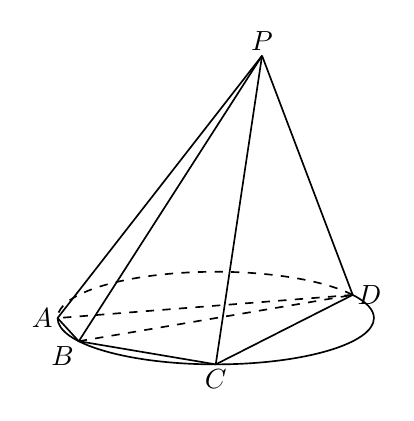
\begin{tikzpicture}[scale=0.98, semithick, every node/.style={inner sep=1.5pt}]
  % 底面椭圆：中心 (2.70,1.15)，半长轴 2.05、半短轴 0.60
  \coordinate (O) at (2.70,1.15);
  \coordinate (A) at (0.65,1.15);
  \coordinate (B) at (0.925,0.85);
  \coordinate (C) at (2.70,0.55);
  \coordinate (D) at (4.475,1.45);
  \coordinate (P) at (3.30,4.55);

  % 底面椭圆：后半（D→上→A）虚线，前半（A→下→D）实线
  \draw[dashed] (D) arc[start angle=30, end angle=180, x radius=2.05, y radius=0.60];
  \draw (A) arc[start angle=180, end angle=390, x radius=2.05, y radius=0.60];

  % 底面四边形的边
  \draw (A) -- (B) -- (C) -- (D);
  \draw[dashed] (D) -- (A);
  \draw[dashed] (B) -- (D);

  % 侧棱
  \draw (P) -- (A);
  \draw (P) -- (B);
  \draw (P) -- (C);
  \draw (P) -- (D);

  \node[above] at (P) {$P$};
  \node[left] at (A) {$A$};
  \node[below left] at (B) {$B$};
  \node[below] at (C) {$C$};
  \node[right] at (D) {$D$};
\end{tikzpicture}
\end{center}
\nopagebreak[4]
\Needspace{4\baselineskip}
\textbf{解析}

（1）$BD$ 为直径，故 $\angle BAD=\angle BCD=90^\circ$。

\Needspace{5\baselineskip}
在 $\mathrm{Rt}\triangle ABD$ 中

\nopagebreak[4]
\[AB=BD\cos60^\circ=R,\qquad AD=BD\sin60^\circ=\sqrt3R.\]

\Needspace{5\baselineskip}
由 $\triangle ADP\sim\triangle BAD$（对应 $A\leftrightarrow B$，$D\leftrightarrow A$，$P\leftrightarrow D$）得

\nopagebreak[4]
\[\frac{AD}{BA}=\frac{DP}{AD}\ \Longrightarrow\ DP=\frac{AD^2}{AB}=\frac{3R^2}{R}=3R.\]

\Needspace{5\baselineskip}
（2）由相似还可得 $\angle ADP=\angle BAD=90^\circ$，即 $PD\perp AD$；且

\nopagebreak[4]
\[AP=\frac{BD\cdot AD}{BA}=\frac{2R\cdot\sqrt3R}{R}=2\sqrt3R.\]

\Needspace{5\baselineskip}
以 $D$ 为原点、$DB$ 为 $x$ 轴建立空间直角坐标系，$A$，$C$ 在 $xy$ 平面内：

\nopagebreak[4]
\[D(0,0,0),\quad B(2R,0,0),\quad A\left(\frac{3R}2,\frac{\sqrt3R}2,0\right),\]

\Needspace{5\baselineskip}
在 $\mathrm{Rt}\triangle BCD$ 中 $\angle BDC=45^\circ$，$CD=\sqrt2R$，且 $C$ 与 $A$ 分居 $BD$ 两侧，

\nopagebreak[4]
\[C(R,-R,0).\]

\Needspace{5\baselineskip}
设 $P(x,y,z)$。由 $PD\perp AD$ 得

\nopagebreak[4]
\[\left(x,y,z\right)\cdot\left(\frac{3R}2,\frac{\sqrt3R}2,0\right)=0\ \Longrightarrow\ 3x+\sqrt3y=0.\]

又 $|PD|=3R$：$x^2+y^2+z^2=9R^2$，与上式联立得 $4x^2+z^2=9R^2$。

\Needspace{5\baselineskip}
由 $|PC|=\sqrt{11}R$：

\nopagebreak[4]
\[(x-R)^2+(y+R)^2+z^2=11R^2.\]

把 $y=-\sqrt3x$ 代入并整理，减去 $4x^2+z^2=9R^2$ 得 $-2(1+\sqrt3)Rx=0$，故 $x=0$，$y=0$，$z=3R$（取上方）。

即 $P$ 在 $D$ 的正上方，到平面 $ABC$ 的距离为 $3R$。

\Needspace{5\baselineskip}
底面 $\triangle ABC$ 中 $AB=R$，$BC=\sqrt2R$，$\angle ABC=\angle ABD+\angle DBC=60^\circ+45^\circ=105^\circ$，

\nopagebreak[4]
\[S_{\triangle ABC}=\frac12\cdot R\cdot\sqrt2R\cdot\sin105^\circ=\frac{\sqrt3+1}4R^2.\]

\Needspace{5\baselineskip}
故

\nopagebreak[4]
\[V_{P-ABC}=\frac13\cdot\frac{\sqrt3+1}4R^2\cdot3R=\frac{\sqrt3+1}4R^3.\]

\gkanswer{答案：（1）$3R$；（2）$\dfrac{\sqrt3+1}4R^3$。}

\end{answer}
\begin{answer}
\gksolhead{19}{}

\textbf{题目}：

某初级中学共有学生 $2000$ 名，各年级男、女生人数如下表：

\begin{center}
\begin{tabular}{llll}
\toprule
 & 一年级 & 二年级 & 三年级 \\
\midrule
女生 & $373$ & $x$ & $y$ \\
男生 & $377$ & $370$ & $z$ \\
\bottomrule
\end{tabular}
\end{center}

已知在全校学生中随机抽取 $1$ 名，抽到初二年级女生的概率是 $0.19$。

（1）求 $x$ 的值；

（2）现用分层抽样的方法在全校抽取 $48$ 名学生，问应在初三年级抽取多少名？

（3）已知 $y\geqslant245$，$z\geqslant245$，求初三年级中女生比男生多的概率。

\Needspace{4\baselineskip}
\textbf{解析}

\Needspace{5\baselineskip}
（1）抽到初二女生的概率为 $\dfrac x{2000}=0.19$，故

\nopagebreak[4]
\[x=380.\]

\Needspace{5\baselineskip}
（2）一年级共 $373+377=750$ 人，二年级共 $380+370=750$ 人，故三年级共

\nopagebreak[4]
\[2000-750-750=500\ \text{\text{人}}.\]

\Needspace{5\baselineskip}
分层抽样应抽

\nopagebreak[4]
\[48\times\frac{500}{2000}=12\ \text{\text{名}}.\]

（3）$y+z=500$，$y\geqslant245$，$z\geqslant245$，故 $y$ 取 $245,246,\cdots,255$ 共 $11$ 个值，等可能。

\Needspace{5\baselineskip}
女生比男生多即 $y>z$，即 $y>250$，$y=251,252,\cdots,255$ 共 $5$ 个值，故

\nopagebreak[4]
\[P=\frac5{11}.\]

\gkanswer{答案：（1）$x=380$；（2）$12$ 名；（3）$\dfrac5{11}$。}

\end{answer}
\begin{answer}
\gksolhead{20}{}

\textbf{题目}：

设 $b>0$，椭圆方程为 $\dfrac{x^2}{2b^2}+\dfrac{y^2}{b^2}=1$，抛物线方程为 $x^2=8(y-b)$。如图所示，过点 $F(0,b+2)$ 作 $x$ 轴的平行线，与抛物线在第一象限的交点为 $G$。已知抛物线在点 $G$ 的切线经过椭圆的右焦点 $F_1$。

（1）求满足条件的椭圆方程和抛物线方程；

（2）设 $A$，$B$ 分别是椭圆长轴的左、右端点，试探究在抛物线上是否存在点 $P$，使得 $\triangle ABP$ 为直角三角形？若存在，请指出共有几个这样的点？并说明理由（不必具体求出这些点的坐标）。
\nopagebreak[4]
\begin{center}% 2008 年广东卷文科第 20 题：椭圆与抛物线，过 F(0,b+2) 作 x 轴的平行线，与抛物线在
%   第一象限的交点为 G，抛物线在 G 处的切线过椭圆的右焦点 F1(b,0)。
% 来源 PDF：gaokaomath-src/普通高考/2008/2008广东文.pdf
% SHA-256：1adedadb12b82b7b4d04721908bd686e747021593ec91da14b0e4e979929373c
% 原页：2008广东文.pdf 第 2 页（A3 三栏）第 2 栏，书页码 448。
% 重绘依据：取 b=1 画示意图：椭圆 x²/2+y²=1，抛物线 x²=8(y-1)，G(4,3)，
%   切线 y=x-1 过 F1(1,0)；A、B 为椭圆长轴端点。
\begin{tikzpicture}[x=1.05cm, y=1.05cm, semithick, font=\small,
  every node/.style={inner sep=1.2pt}]
  \draw[->,>=stealth] (-4.7,0) -- (5.6,0) node[right] {$x$};
  \draw[->,>=stealth] (0,-1.4) -- (0,5.6) node[above] {$y$};
  \node[below left] at (0,0) {$O$};

  % 椭圆 x^2/2 + y^2 = 1
  \draw[line width=0.9pt] (0,0) ellipse (1.414 and 1);
  \node[below left] at (-1.414,0) {$A$};
  \node[below right] at (1.414,0) {$B$};
  \fill (1,0) circle (1.2pt) node[above left] {$F_1$};

  % 抛物线 x^2 = 8(y-1)
  \draw[line width=0.9pt, domain=-4.35:4.35, samples=140] plot (\x, {(\x*\x)/8+1});

  % 过 F(0,3) 的水平线与 G(4,3)
  \draw (-4.5,3) -- (5.2,3);
  \node[above left=2pt] at (0,3) {$F$};
  \fill (4,3) circle (1.2pt) node[above left=1pt] {$G$};

  % 抛物线在 G 处的切线 y = x - 1
  \draw (0.9,-0.1) -- (5.2,4.2);
\end{tikzpicture}
\end{center}
\nopagebreak[4]
\Needspace{4\baselineskip}
\textbf{解析}

（1）$y=b+2$ 与 $x^2=8(y-b)$ 联立：$x^2=8\cdot2=16$，在第一象限得 $G(4,b+2)$。

\Needspace{5\baselineskip}
抛物线 $x^2=8(y-b)$ 在 $G$ 处切线斜率 $y'=\dfrac x4\Big|_{x=4}=1$，切线为

\nopagebreak[4]
\[y-(b+2)=x-4,\qquad\text{\text{即} }y=x+b-2.\]

椭圆 $\dfrac{x^2}{2b^2}+\dfrac{y^2}{b^2}=1$ 中 $c^2=2b^2-b^2=b^2$，右焦点 $F_1(b,0)$。

\Needspace{5\baselineskip}
切线过 $F_1$：

\nopagebreak[4]
\[0=b+b-2\ \Longrightarrow\ b=1.\]

故椭圆为 $\dfrac{x^2}2+y^2=1$，抛物线为 $x^2=8(y-1)$。

（2）存在，共 $4$ 个。理由如下。

$A(-\sqrt2,0)$，$B(\sqrt2,0)$，抛物线上点 $P\left(t,\dfrac{t^2}8+1\right)$，其中 $\dfrac{t^2}8+1>0$。

① 直角在 $A$ 处：$AP\perp AB$，而 $AB$ 沿 $x$ 轴，故 $AP$ 竖直，$x_P=-\sqrt2$，得唯一一点。

② 直角在 $B$ 处：同理 $x_P=\sqrt2$，得唯一一点。

\Needspace{5\baselineskip}
③ 直角在 $P$ 处：$\overrightarrow{PA}\cdot\overrightarrow{PB}=0$，即

\nopagebreak[4]
\[\overrightarrow{PA}\cdot\overrightarrow{PB}=\left(-\sqrt2-t\right)\left(\sqrt2-t\right)+y^2=\left(t^2-2\right)+y^2=0,\]

\Needspace{5\baselineskip}
即 $y^2=2-t^2$。代入 $y=\dfrac{t^2}8+1$，令 $u=t^2\geqslant0$：

\nopagebreak[4]
\[\left(\frac u8+1\right)^2=2-u\ \Longrightarrow\ u^2+80u-64=0,\]

其正根 $u=\dfrac{-80+\sqrt{6656}}2=\dfrac{-80+16\sqrt{26}}2=-40+8\sqrt{26}\approx0.81$，对应 $t=\pm\sqrt u$ 两点。

综上，共有 $1+1+2=4$ 个点。

\gkanswer{答案：（1）$\dfrac{x^2}2+y^2=1$，$x^2=8(y-1)$；（2）存在，共 $4$ 个。}

\end{answer}
\begin{answer}
\gksolhead{21}{}

\textbf{题目}：

设数列 $\{a_n\}$ 满足 $a_1=1$，$a_2=2$，$a_n=\dfrac13\left(a_{n-1}+2a_{n-2}\right)$（$n=3,4,\cdots$）。数列 $\{b_n\}$ 满足 $b_1=1$，$b_n$（$n=2,3,\cdots$）是非零整数，且对任意的正整数 $m$ 和自然数 $k$，都有 $-1\leqslant b_m+b_{m+1}+\cdots+b_{m+k}\leqslant1$。

（1）求数列 $\{a_n\}$ 和 $\{b_n\}$ 的通项公式；

（2）若 $c_n=na_nb_n$（$n=1,2,\cdots$），求数列 $\{c_n\}$ 的前 $n$ 项和 $S_n$。

\Needspace{4\baselineskip}
\textbf{解析}

（1）由 $3a_n=a_{n-1}+2a_{n-2}$ 得特征方程 $3r^2=r+2$，即 $3r^2-r-2=0$，根为 $r=1$，$r=-\dfrac23$。

\Needspace{5\baselineskip}
设 $a_n=A+B\left(-\dfrac23\right)^{n-1}$，由 $a_1=1$，$a_2=2$：

\nopagebreak[4]
\[A+B=1,\qquad A-\frac23B=2,\]

\Needspace{5\baselineskip}
相减得 $\dfrac53B=-1$，$B=-\dfrac35$，$A=\dfrac85$，故

\nopagebreak[4]
\[a_n=\frac85-\frac35\left(-\frac23\right)^{n-1}.\]

（$b_n$）$b_n$ 均为非零整数，取 $k=0$ 得 $-1\leqslant b_m\leqslant1$，故 $b_m=\pm1$；

取 $k=1$ 得 $-1\leqslant b_m+b_{m+1}\leqslant1$，而 $b_m$，$b_{m+1}\in\{-1,1\}$，故只能 $b_{m+1}=-b_m$。

\Needspace{5\baselineskip}
由 $b_1=1$ 得

\nopagebreak[4]
\[b_n=(-1)^{n-1}.\]

（可直接验证：任意连续若干项之和为 $0$、$1$ 或 $-1$，满足条件。）

\Needspace{5\baselineskip}
（2）$c_n=na_nb_n$，记 $q=\dfrac23$、$T_1=\sum\limits_{k=1}^nk(-1)^{k-1}$，则

\nopagebreak[4]
\[c_k=\frac85k(-1)^{k-1}-\frac35k(-1)^{k-1}\left(-\frac23\right)^{k-1}=\frac85k(-1)^{k-1}-\frac35kq^{k-1}.\]

\Needspace{5\baselineskip}
求和并用 $\sum\limits_{k=1}^nkq^{k-1}=9-3(n+3)q^n$：

\nopagebreak[4]
\[S_n=\frac85T_1-\frac35\left[9-3(n+3)q^n\right]=\frac85T_1-\frac{27}5+\frac95(n+3)\left(\frac23\right)^n.\]

\Needspace{5\baselineskip}
其中

\nopagebreak[4]
\[T_1=\begin{cases}-\dfrac n2,&n\text{ \text{为偶数}},\\[4pt]\dfrac{n+1}2,&n\text{ \text{为奇数}}.\end{cases}\]

\Needspace{5\baselineskip}
故

\nopagebreak[4]
\[S_n=\begin{cases}-\dfrac{4n+27}5+\dfrac95(n+3)\left(\dfrac23\right)^n,&n\text{ \text{为偶数}},\\[8pt]\dfrac{4n-23}5+\dfrac95(n+3)\left(\dfrac23\right)^n,&n\text{ \text{为奇数}}.\end{cases}\]

\gkanswer{答案：（1）$a_n=\dfrac85-\dfrac35\left(-\dfrac23\right)^{n-1}$，$b_n=(-1)^{n-1}$；（2）见解析。}

\end{answer}